% fig_ibr_coverage_map.tex
% TR-29: Coverage map on (alpha, k_ibr) plane
%
% X-axis: fault location alpha in [0, 1.0]
% Y-axis: IBR current limit k_ibr in [0.06, 0.20]
%
% Coverage regions:
%   Region A (RED):    k_ibr < 0.10, all alpha
%                      Distance relay BLOCKED (I < I_min = 0.10 pu)
%                      87L chain: TDCS sole instantaneous detector
%
%   Region B (AMBER):  k_ibr >= 0.10, alpha > 0.80
%                      Distance relay: Zone 2 asserted but memory expires
%                      before 300 ms timer -> Zone 2 trip FAILS
%                      87L chain: TDCS instantaneous sole detector
%
%   Region C (GREEN):  k_ibr in [0.10, 0.12), alpha <= 0.80
%                      Distance relay: Zone 1 within memory window -> trips
%                      87L chain: TDCS (87L element below threshold)
%                      Dual redundancy (both elements detect)
%
%   Region D (DARK GREEN): k_ibr >= 0.12, alpha <= 0.80
%                      Distance relay: Zone 1 within memory window -> trips
%                      87L chain: 87L element + TDCS
%                      Full dual redundancy
%
% Key boundaries:
%   k_ibr = 0.10: I_min threshold (horizontal)
%   k_ibr = 0.12: 87L element threshold (horizontal dashed)
%   alpha = 0.80: Zone 1 / Zone 2 boundary (vertical)

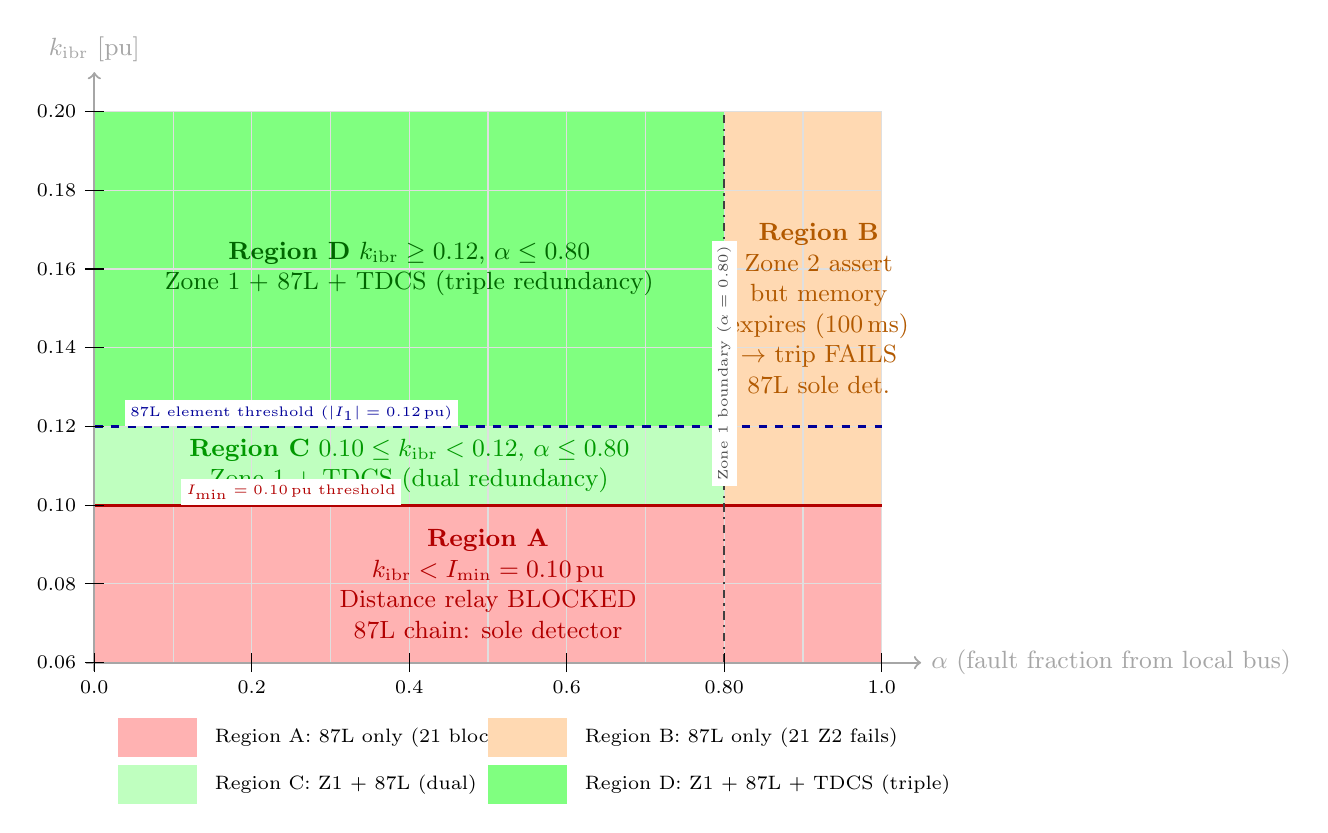
\begin{tikzpicture}[
  every node/.style={font=\scriptsize},
]

% ---- Coordinate scaling: alpha [0,1] -> x [0,10], k_ibr [0.06,0.20] -> y [0,7] ----
% x = alpha * 10
% y = (k_ibr - 0.06) / 0.14 * 7

% Region A: k_ibr < 0.10 -> y < (0.10-0.06)/0.14*7 = 2.0
\fill[red!30] (0,0) rectangle (10, 2.0);

% Region B: k_ibr >= 0.10, alpha > 0.80 -> x > 8.0, y >= 2.0
\fill[orange!30] (8.0, 2.0) rectangle (10, 7.0);

% Region C: k_ibr in [0.10, 0.12), alpha <= 0.80 -> y in [2.0, 3.0), x <= 8.0
\fill[green!25] (0, 2.0) rectangle (8.0, 3.0);

% Region D: k_ibr >= 0.12, alpha <= 0.80 -> y >= 3.0, x <= 8.0
\fill[green!50] (0, 3.0) rectangle (8.0, 7.0);

% ---- Grid ----
\draw[gray!25, step=1.0] (0,0) grid (10,7);

% ---- Boundary lines ----
% k_ibr = 0.10 (I_min threshold): y = 2.0
\draw[red!70!black, very thick] (0, 2.0) -- (10, 2.0);

% k_ibr = 0.12 (87L element threshold): y = 3.0
\draw[blue!60!black, thick, dashed] (0, 3.0) -- (10, 3.0);

% alpha = 0.80 (Zone 1 / Zone 2 boundary): x = 8.0
\draw[gray!50!black, thick, dash dot] (8.0, 0) -- (8.0, 7.0);

% ---- Axes ----
\draw[->, thick, gray!70] (-0.1, 0) -- (10.5, 0)
  node[right, font=\small] {$\alpha$ (fault fraction from local bus)};
\draw[->, thick, gray!70] (0, -0.1) -- (0, 7.5)
  node[above, font=\small] {$k_{\rm ibr}$ [pu]};

% ---- X-axis ticks ----
\foreach \a/\x in {0.0/0, 0.2/2, 0.4/4, 0.6/6, 0.80/8, 1.0/10} {
  \draw (\x, -0.12) -- (\x, 0.12);
  \node[below=3pt] at (\x, 0) {\a};
}

% ---- Y-axis ticks ----
\foreach \k/\y/\label in {
  0.06/0.0/0.06,
  0.08/1.0/0.08,
  0.10/2.0/0.10,
  0.12/3.0/0.12,
  0.14/4.0/0.14,
  0.16/5.0/0.16,
  0.18/6.0/0.18,
  0.20/7.0/0.20
} {
  \draw (-0.12, \y) -- (0.12, \y);
  \node[left=3pt] at (0, \y) {\label};
}

% ---- Region labels ----
% Region A
\node[align=center, red!70!black, font=\small] at (5.0, 1.0) {
  \textbf{Region A}\\
  $k_{\rm ibr} < I_{\rm min} = 0.10$\,pu\\
  Distance relay BLOCKED\\
  87L chain: sole detector};

% Region B
\node[align=center, orange!70!black, font=\small] at (9.2, 4.5) {
  \textbf{Region B}\\
  Zone 2 assert\\
  but memory\\
  expires (100\,ms)\\
  $\to$ trip FAILS\\
  87L sole det.};

% Region C
\node[align=center, green!60!black, font=\small] at (4.0, 2.5) {
  \textbf{Region C}  $0.10 \leq k_{\rm ibr} < 0.12$, $\alpha \leq 0.80$\\
  Zone 1 + TDCS  (dual redundancy)};

% Region D
\node[align=center, green!40!black, font=\small] at (4.0, 5.0) {
  \textbf{Region D}  $k_{\rm ibr} \geq 0.12$, $\alpha \leq 0.80$\\
  Zone 1 + 87L + TDCS  (triple redundancy)};

% ---- Boundary annotations ----
\node[red!70!black, fill=white, inner sep=2pt, font=\tiny]
  at (2.5, 2.0) [above] {$I_{\rm min} = 0.10$\,pu threshold};

\node[blue!60!black, fill=white, inner sep=2pt, font=\tiny]
  at (2.5, 3.0) [above] {87L element threshold ($|I_1| = 0.12$\,pu)};

\node[gray!60!black, fill=white, inner sep=2pt, font=\tiny,
      rotate=90] at (8.0, 3.8) {Zone 1 boundary ($\alpha=0.80$)};

% ---- Legend ----
\fill[red!30]    (0.3, -1.2) rectangle (1.3, -0.7);
\node[right=3pt] at (1.3, -0.95) {Region A: 87L only (21 blocked)};
\fill[orange!30] (5.0, -1.2) rectangle (6.0, -0.7);
\node[right=3pt] at (6.0, -0.95) {Region B: 87L only (21 Z2 fails)};

\fill[green!25]  (0.3, -1.8) rectangle (1.3, -1.3);
\node[right=3pt] at (1.3, -1.55) {Region C: Z1 + 87L (dual)};
\fill[green!50]  (5.0, -1.8) rectangle (6.0, -1.3);
\node[right=3pt] at (6.0, -1.55) {Region D: Z1 + 87L + TDCS (triple)};

\end{tikzpicture}
